\documentclass[fleqn]{hw}

\usepackage{notes}
\usepackage{url}
\usepackage{graphicx}
\usepackage{amsmath}
\title{HW3: Markov Decision Processes}
\duedate{}
\class{CS6300: Artificial Intelligence, Spring 2018}
\institute{University of Utah}
\author{Jake Pitkin}
% IF YOU'RE USING THIS .TEX FILE AS A TEMPLATE, PLEASE REPLACE
% The author WITH YOUR NAME AND UID.
% Replace the due date with anyone you worked with i.e. "Worked with: John McCarthy, Watson, & Hal-9000"
\begin{document}
\maketitle

% IF YOU'RE USING THIS .TEX FILE AS A TEMPLATE, PLEASE REPLACE
% "CS5300, Spring 2009" WITH YOUR NAME AND UID.

% Hand in at: http://www.cs.utah.edu/~hal/handin.pl?course=cs5300

\section{Life as a Professor}

Bob, our venerable AI professor, is currently riding the currents of
new-professorhood.  To better understand what his life will be like,
he has constructed a Markov Process (note: no actions!) to represent the life of a professor.
He has drawn the life of a professor in the following MP, where rewards are written on the states
and transition probabilities are written on the arcs.  His start state
is as an assistant professor.

\begin{centering}
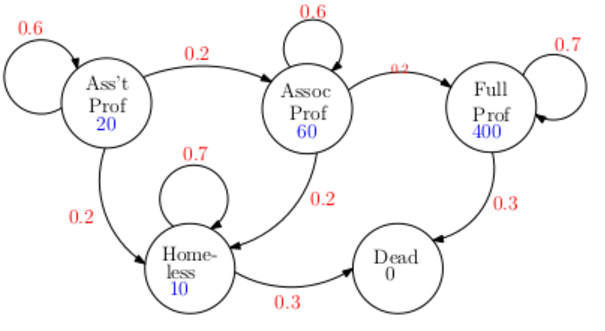
\includegraphics[width=0.8\textwidth]{academic-life.pdf}  
\end{centering}

\begin{enumerate}

\item Fill in the following table with the $V^*$ values for each state in
the MDP for $t = 1 \dots 5$; I have filled in the first three values
to help you out (hint: use the value iteration Bellman updates, but
remove the ``$\max_a$'' part because you don't need to select
actions).  Suppose $\gamma = 0.5$.

\begin{tabular}{|c||c|c|c|c|c|}
\hline
{\bf t} & $V_t^*(\text{asst})$ & $V_t^*(\text{assc})$ & $V_t^*(\text{full})$ & $V_t^*(\text{hl})$ & $V_t^*(\text{dead})$ \\
\hline
$0$ & $0$ & $0$ & $0$ & $0$ & $0$ \\
\hline
$1$ & $20$ & $60$ & $400$ & $\dots$ & $\dots$ \\
\hline
$2$ & $\dots$ & $\dots$ & $\dots$ & $\dots$ & $\dots$ \\
\hline
$3$ & $\dots$ & $\dots$ & $\dots$ & $\dots$ & $\dots$ \\
\hline
$4$ & $\dots$ & $\dots$ & $\dots$ & $\dots$ & $\dots$ \\
\hline
$5$ & $\dots$ & $\dots$ & $\dots$ & $\dots$ & $\dots$ \\
\hline
\end{tabular}

\item What was the change in max-norm of $V$ between steps $4$ and $5$?  What does this tell us about how close the final values are to the true values?

\end{enumerate}

\newpage

\section{Clarence the Evil Professor}

Alice is also taken another class (class name withheld!) from
Professor Clarence.  Clarence is known to be evil among the department
because he only passes students who sweettalk him.  Based on what
she's learned in AI, Alice has figured out that classes with Clarence
can be modeled with the following MDP:

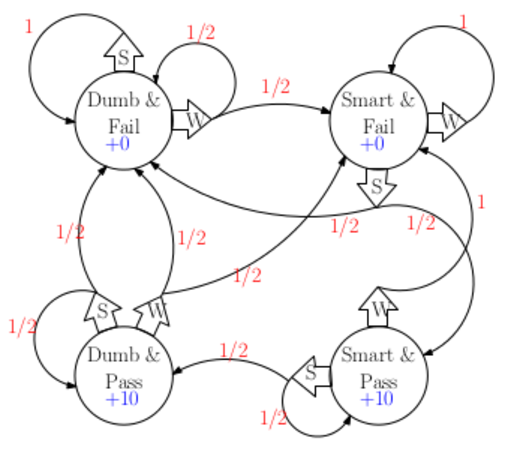
\includegraphics[width=0.8\textwidth]{mdp.pdf}

The difference between this Figure and the one from the previous
question is now Alice has actions she can take.  In any state, she can
either take action ``S'' (to try to \emph{Sweettalk} Clarence) or action
``W'' (to \emph{Work} hard).  Her state is represented by a pair: she can
either be smart or dumb, and she can either pass or fail the course.
The transitions can be read as follows.  If Alice is \emph{Dumb and Failing},
and she chooses to \emph{Sweettalk}, then Clarence won't listen to her
because she's dumb, so with probability $1$ she winds back up in the
same state.  On the other hand, had she chosen to \emph{Work}, then with
$50\%$ probability she'd be successful and become \emph{Smart} (but still
\emph{Failing}) and with $50\%$ probability she'd have studied the wrong
thing and will remain \emph{Dumb and Failing}.

Please answer the following questions with respect to this MDP; always
assume $\gamma = 0.5$:

\begin{enumerate}

\item Suppose that Alice's policy is to always work.  Compute the value
of each state under this policy, running $4$ iterations of value
iterations.  Does this outcome make sense?

\begin{tabular}{|c||c|c|c|c|}
\hline
{\bf t} & D+F & S+F & D+P & S+P \\
\hline
$0$ & $0$ & $0$ & $0$  & $0$  \\
\hline
$1$ & $\dots$ & $\dots$ & $\dots$ & $\dots$ \\
\hline
$2$ & $\dots$ & $\dots$ & $\dots$ & $\dots$ \\
\hline
$3$ & $\dots$ & $\dots$ & $\dots$ & $\dots$ \\
\hline
$4$ & $\dots$ & $\dots$ & $\dots$ & $\dots$ \\
\hline
\end{tabular}

\item Suppose that Alice's policy is to work only when she's dumb and sweettalk when she's smart.
Compute the values here for four steps.  Which policy is better (and
does this make sense)?


\begin{tabular}{|c||c|c|c|c|}
\hline
{\bf t} & D+F & S+F & D+P & S+P \\
\hline
$0$ & $0$ & $0$ & $0$  & $0$  \\
\hline
$1$ & $\dots$ & $\dots$ & $\dots$ & $\dots$ \\
\hline
$2$ & $\dots$ & $\dots$ & $\dots$ & $\dots$ \\
\hline
$3$ & $\dots$ & $\dots$ & $\dots$ & $\dots$ \\
\hline
$4$ & $\dots$ & $\dots$ & $\dots$ & $\dots$ \\
\hline
\end{tabular}

\item Now, suppose we do not begin with an initial policy but just run
plain value iteration.  Show the $V$ values derived through value
iteration for the first four time steps; fill in the table below:

\begin{tabular}{|c||c|c|c|c|}
\hline
{\bf t} & D+F & S+F & D+P & S+P \\
\hline
$0$ & $0$ & $0$ & $0$  & $0$  \\
\hline
$1$ & $0$ & $0$ & $10$ & $10$ \\
\hline
$2$ & $\dots$ & $\dots$ & $\dots$ & $\dots$ \\
\hline
$3$ & $\dots$ & $\dots$ & $\dots$ & $\dots$ \\
\hline
$4$ & $\dots$ & $\dots$ & $\dots$ & $\dots$ \\
\hline
\end{tabular}

\item Let's do policy iteration!  Suppose that Alice
begins with the policy from question (1): always work.  You've already
computed values under this policy.  Use that to estimate a new policy.
Write that policy down.  Compute four iterations of values for that
new policy and compute a third policy.  Has the policy converged?
Does it seem (intuitively) optimal?

\end{enumerate}

\end{document}
